\section{Introduction}

This is a guide for setting up the Android Development environment on Windows. The process is outlined at Google's instructions\sidenote{\url{http://developer.android.com/sdk/installing.html}} and also at Android Development\sidenote{\url{http://learnaboutandroid.blogspot.com/2011/05/setting-up-your-androidjava-environment.html}} (this is 
catered for Mac OS X only, however).

By the end of this you will have Eclipse setup to develop on real Android devices or a virtual Android device.

\section{Downloading}

The first thing that we need to do is to download the following components:
\begin{itemize}
	\item Java SDK
	\item Eclipse IDE
	\item Android SDK
\end{itemize}

The links for these appear in the side note. It's a good idea to start them all downloading at the beginning so as not to waste time.

\subsection{Java SDK}

Download the Java SDK from Oracle's website\sidenote{\url{http://www.oracle.com/technetwork/java/javase/downloads/index.html}} and install.

\begin{figure}[!ht]
  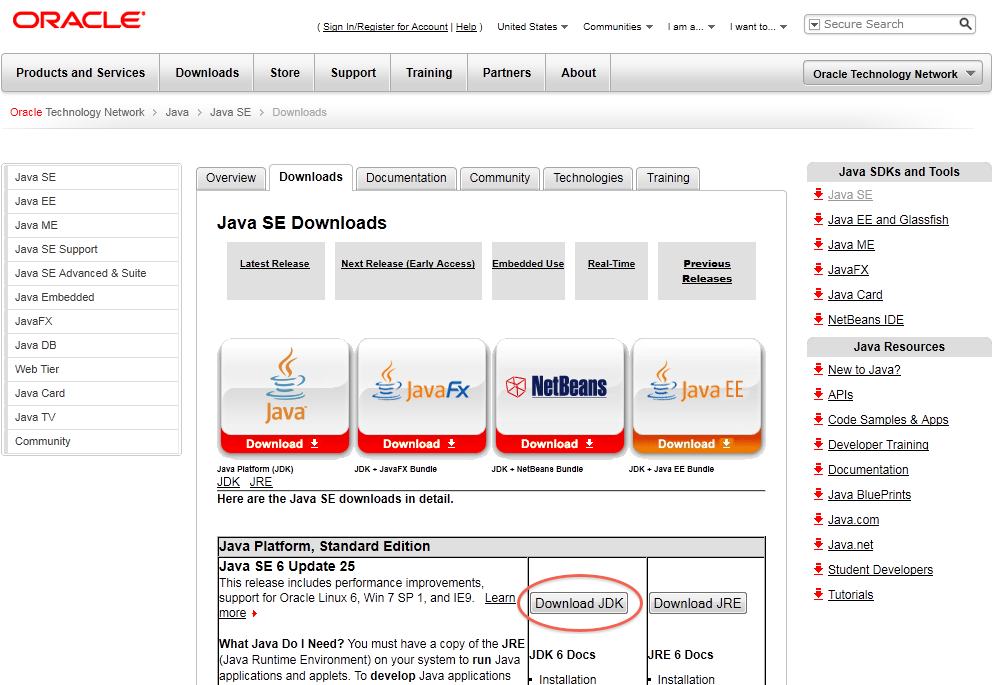
\includegraphics[width=\textwidth]{./images/java_sdk.png}%
  \caption{Download the Java SDK, select the highlighted option.}%
  \label{fig:javasdk}%
\end{figure}

\subsection{Eclipse IDE}

You only need the basic version of Eclipse\sidenote{\url{http://www.eclipse.org/downloads}} (Google recommend the `classic' version).
\begin{figure}[!ht]
  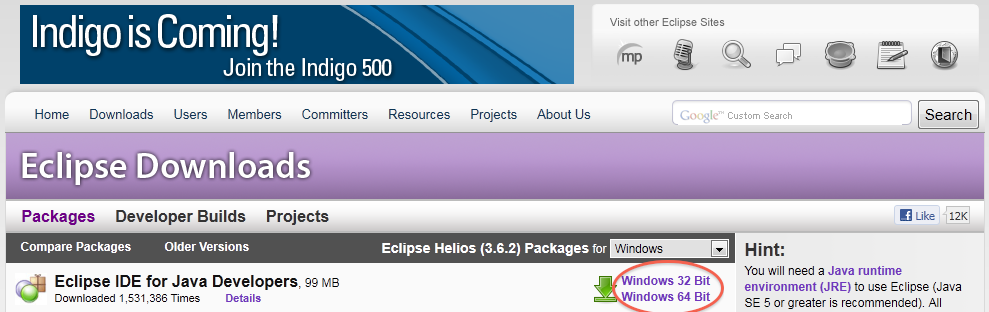
\includegraphics[width=\textwidth]{./images/eclipse.png}%
  \caption{Download Eclipse, select the highlighted option.}%
  \label{fig:eclipseide}%
\end{figure}

You can just extract the contents to your \Verb|C:\Program Files(x86)\| and make a shortcut to \Verb|eclipse.exe| on your desktop.

\subsection{Android SDK}

Download the installer\sidenote{\url{http://developer.android.com/sdk/index.html}} and run it. It will install \newline
to \Verb|C:\Program Files(x86)\Android|. If you decided to change this location, make a note of it because we will need it later when we come to setup Eclipse.

\begin{figure}[!ht]
  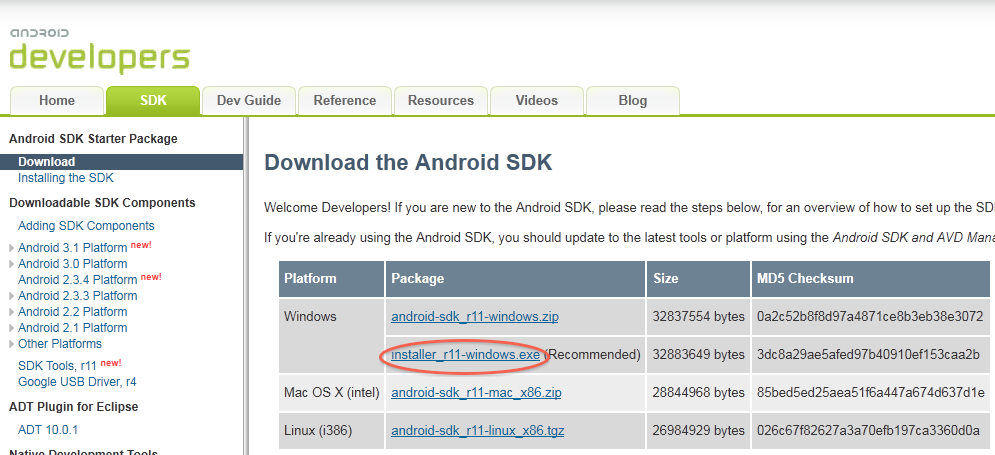
\includegraphics[width=\textwidth]{./images/android.png}%
  \caption{Download Android SDK, select the highlighted option.}%
  \label{fig:androidsdk}%
\end{figure}

Once the installer has finished it's work, let it start the \textbf{SDK Manager} for you. A window will pop up and ask which packages you want to install.
According to Google's Device Chart \ref{fig:device_chart}, the most common devices are running 2.2 and 2.1. Select these from the list. Ensure that the \emph{Google USB Driver package} is selected too \ref{fig:windows_usb_driver}.

\begin{figure}[!ht]
  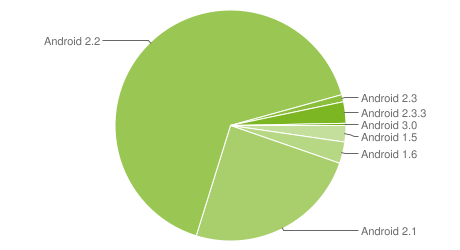
\includegraphics[width=\textwidth]{./images/device_chart.png}%
  \caption{Distribution of Android handsets, retrieved May 28 2011
  \emph{Source: \url{http://developer.android.com/resources/dashboard/platform-versions.html}}}%
  \label{fig:device_chart}%
\end{figure}

\begin{figure}[!ht]
  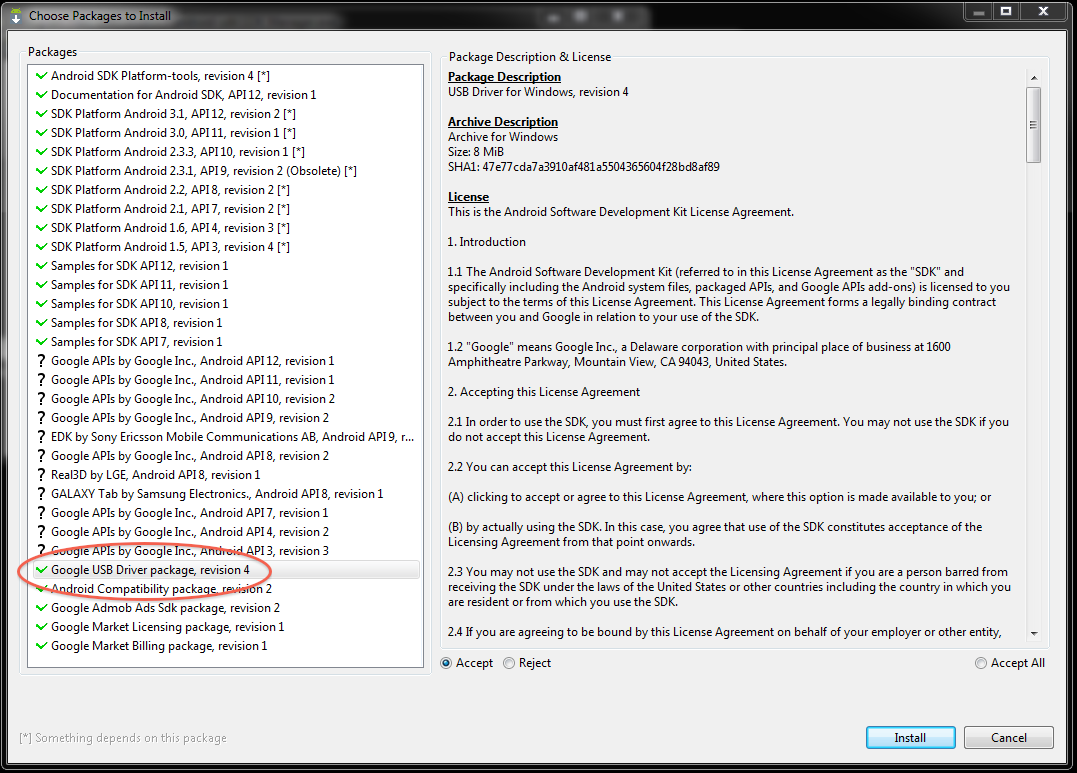
\includegraphics[width=\textwidth]{./images/windows_usb_driver.png}%
  \caption{Android SDK package selection --- ensure the \emph{Google USB Driver package} is selected}%
  \label{fig:windows_usb_driver}
\end{figure}

\section{Eclipse Setup}

There still a little bit more work to do before being able to develop for the phones. We need to install the ADT plugin for Eclipse.

Open Eclipse and select a workspace. This is where your source code will live.

\begin{figure}[!ht]
  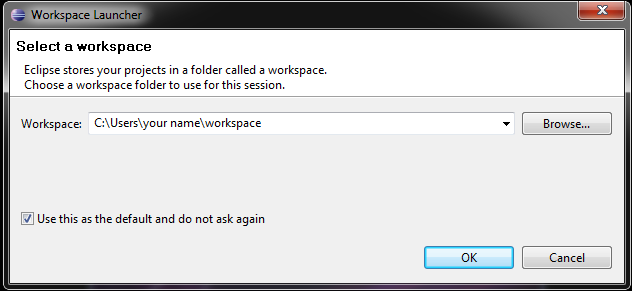
\includegraphics[width=\textwidth]{./images/workspace.png}%
  \caption{By default it'll substitute your name in there, you can select this workspace by default every time you open Eclipse}
  \label{fig:workspace}
\end{figure}

Once you have selected a workspace the next screen you'll see is this:

\begin{figure}[!ht]
  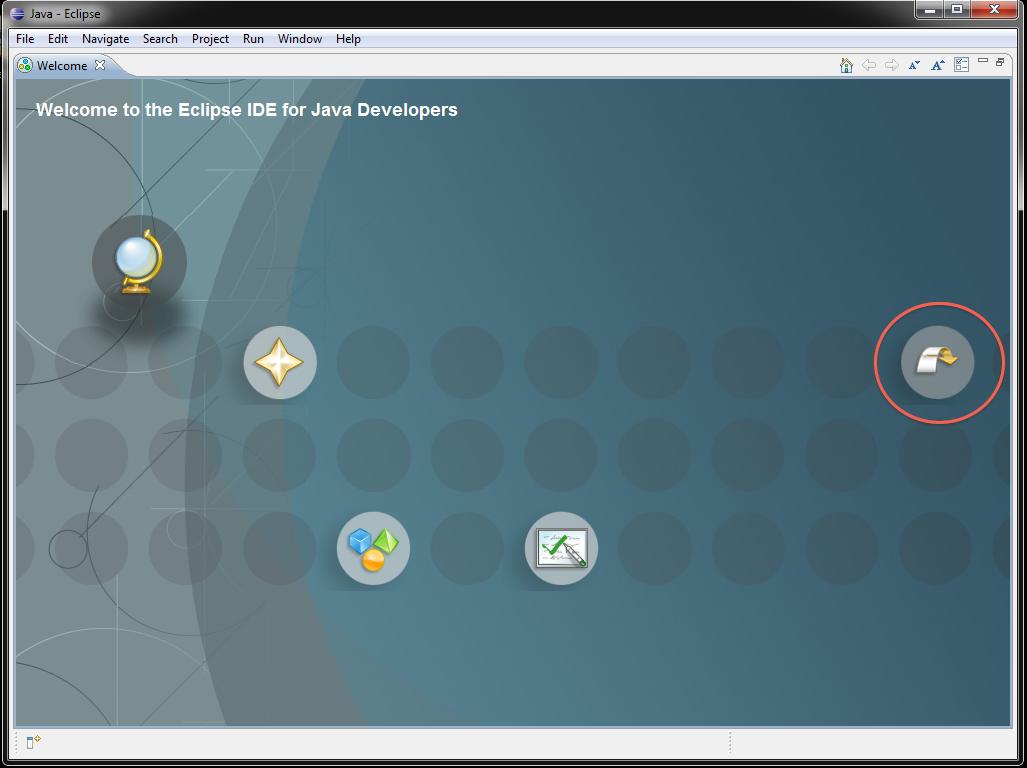
\includegraphics[width=\textwidth]{./images/go_to_workbench.png}%
  \caption{Eclipse's Opening Screen}
  \label{fig:workbench}
\end{figure}

Select the arrow icon on the right to go to the workbench. On the left of the workbench is where your projects end up, for the moment it'll be empty (you've not created anything yet!). The portion in the middle is where the code will appear.

To install the plugin, go to \textit{Help} and select \textit{Install New Software}. Click on the \textit{Add} button. You will need to enter the information as in \ref{fig:new_software}. Once you've added that information you will see the list populated with items that can be installed. Select the \textit{Developer Tools} and proceed with the installation.

\begin{figure}[!ht]
  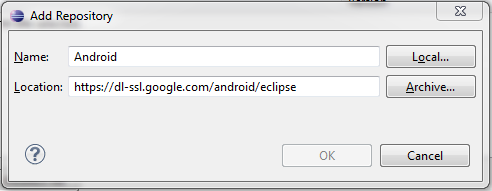
\includegraphics[width=\textwidth]{./images/new_software.png}%
  \caption{Adding a new software source to Eclipse}
  \label{fig:new_software}
\end{figure}

\begin{figure}[!ht]
  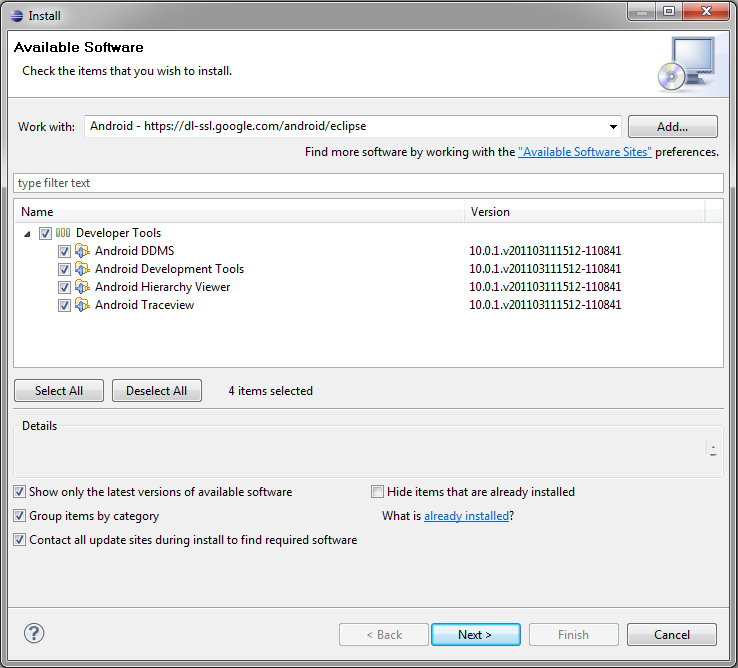
\includegraphics[width=\textwidth]{./images/adt_plugin.png}%
  \caption{Proceeding with the installation}
  \label{fig:adt_plugin}
\end{figure}

Eclipse will ask to restart after the plugins have been installed. Allow it to restart. When you open Eclipse you will see a new menu icon \ref{fig:adt_success}. This means that the plugin has installed successfully.

\begin{figure}[!ht]
  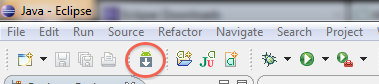
\includegraphics[width=\textwidth]{./images/success.png}%
  \caption{Plugin installation success!}
  \label{fig:adt_success}
\end{figure}

The last thing that we need to do is to tell Eclipse where to find the SDK. To do this, click on \textit{Preferences} and under \textit{Android} there is a box there for the SDK Location. Click the \textit{edit} button, and navigate to the path where the SDK was installed, by default it is \newline
\Verb|C:\Program Files(x86)\Android\android-sdk|.\sidenote{If you've changed this in a previous step, put the changed path here.} Click \textit{Apply}, you should see the list of available targets update.

\begin{figure}[!ht]
  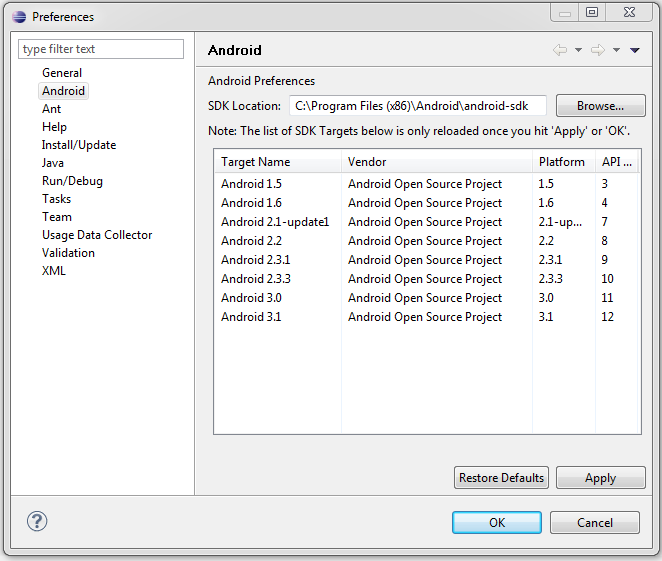
\includegraphics[width=\textwidth]{./images/sdk_location.png}%
  \caption{Locating the Android SDK for Eclipse}
  \label{fig:find_android_sdk}
\end{figure}

\section{Developing}

There are two paths from here. You can develop using an emulated device or with a real one. The problem with the emulation is that there isn't an easy way to test sensors and accelerometer based applications.

We'll first setup a virtual device then move on to the real device setup. Finally, we'll get a basic `Hello World!' project started.

\subsection{Virtual Devices}

If you click on the icon in \ref{fig:adt_success} you'll be presented with an AVD manager. Click on the \textit{New} button on the right hand side, and create an AVD. When it comes to naming it's a good idea to name it something meaningful, here we use the version number of the target (so we know instantly which device we can deploy on).

\begin{figure}[!ht]
  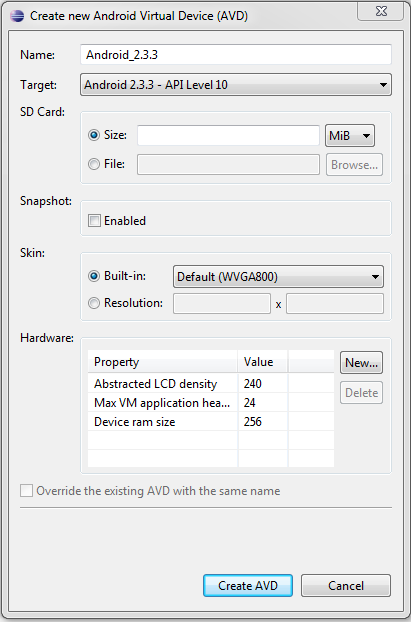
\includegraphics[width=\textwidth]{./images/new_avd.png}%
  \caption{Creating a new Android Virtual Device}
  \label{fig:new_avd}
\end{figure}

Once you've created the device, you can start it up. You may have to wait.

\begin{figure}[!ht]
  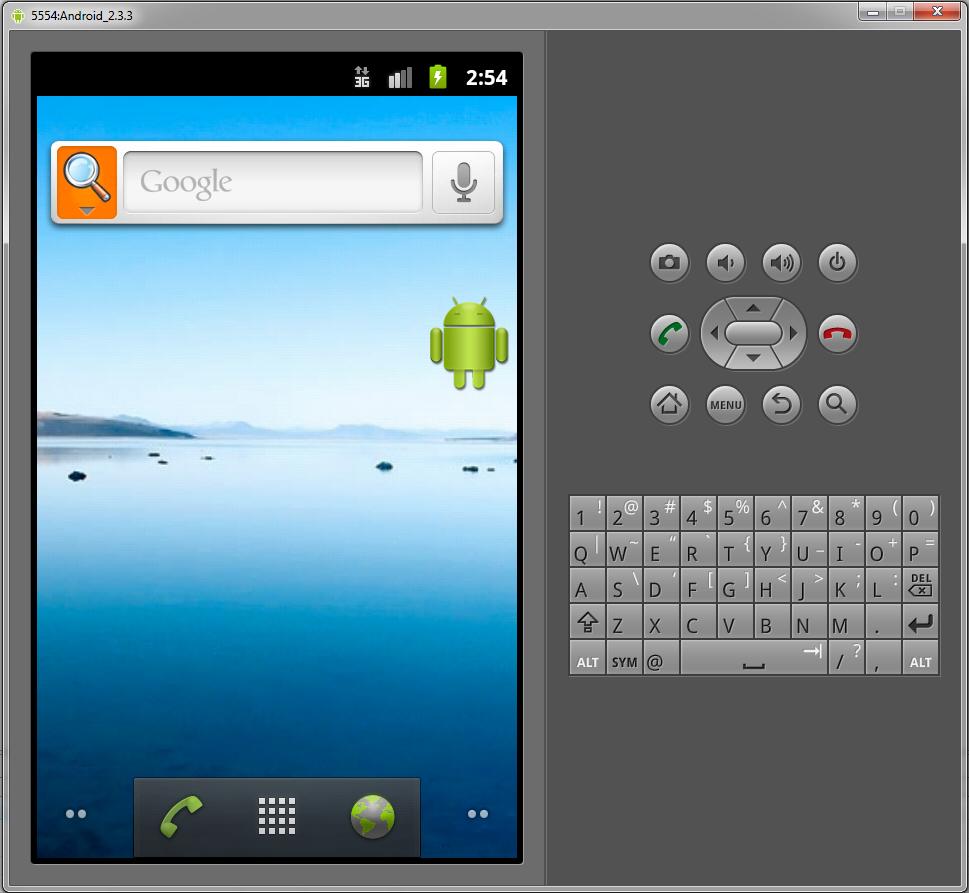
\includegraphics[width=\textwidth]{./images/avd.png}%
  \caption{Running the Android Virtual Device}
  \label{fig:avd}
\end{figure}

\clearpage

\subsection{Real Devices}

For developing on Windows with real devices you need to jump through another couple of hoops that are unnecessary for Mac and Linux platforms.

Plug your phone in via it's USB cable. Windows will try to find drivers for it. Depending on the phone it may succeed --- for the Nexus S, it didn't. In order to install the drivers, you need to right click on \textit{Computer} (in the \textit{Start Menu}), and select \textit{Manage}. Select the \textit{Device Manager} from the next window. 

\begin{figure}[!ht]
  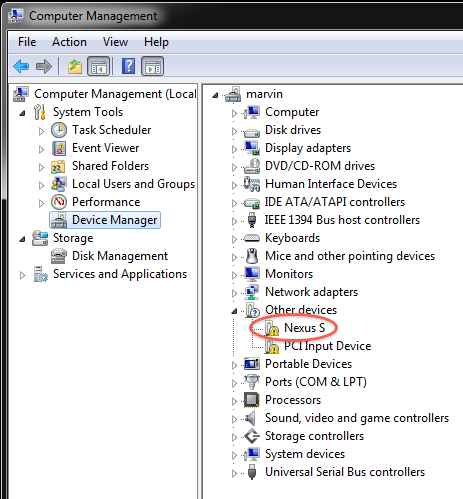
\includegraphics[width=\textwidth]{./images/device_manager.png}%
  \caption{Device Manager with the driverless Android Phone}
  \label{fig:device_manager}
\end{figure}

If you expand \textit{Other Devices} you should see your phone listed there. Right click your phone, and select \textit{Update Driver Software} and navigate to \Verb|C:\Program Files(x86)\Android\android-sdk\extras\google\usb_driver|. Allow the installation process to proceed. 

\begin{figure}[!ht]
  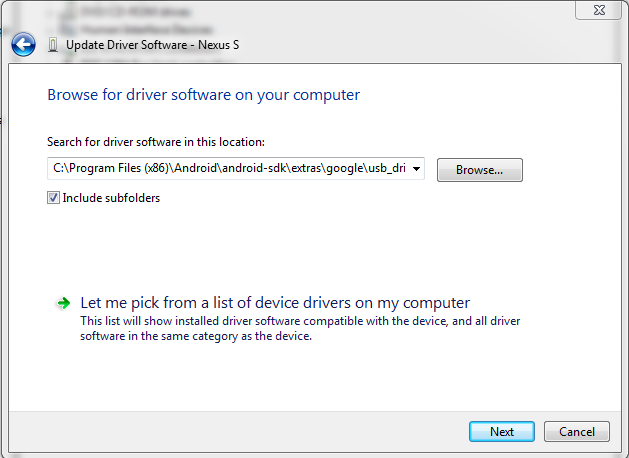
\includegraphics[width=\textwidth]{./images/browse_drivers.png}%
  \caption{Browsing for the drivers for the phone}
  \label{fig:browse_driver}
\end{figure}

\begin{figure}[!ht]
  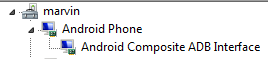
\includegraphics[width=\textwidth]{./images/driver_success.png}%
  \caption{Successful installation of the USB driver}
  \label{fig:success_driver}
\end{figure}

\clearpage

\subsection{Hello World!}

In Eclipse, start a new \textit{Other Project}, and use the \textit{Android Project} wizard. Fill out the fields according to \ref{fig:new_project} and it'll appear in the \textit{Package Explorer}. 

\begin{figure}[!ht]
  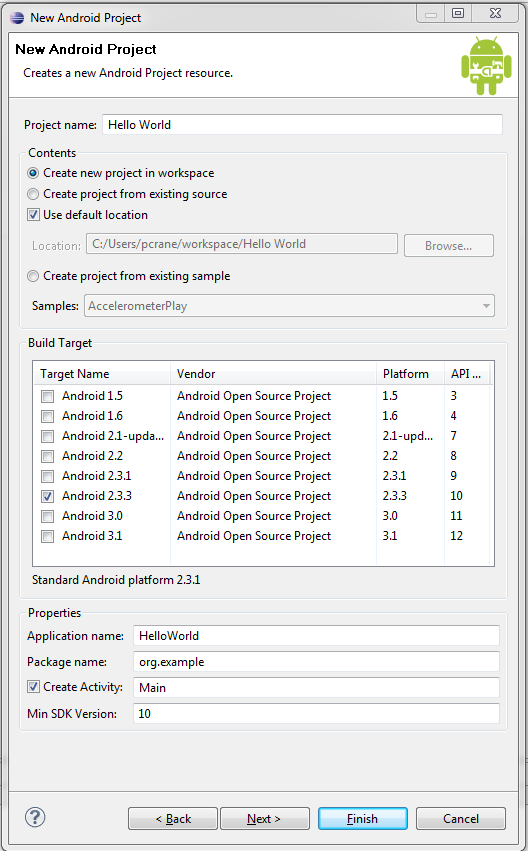
\includegraphics[width=\textwidth]{./images/new_project.png}%
  \caption{Successful installation of the USB driver}
  \label{fig:new_project}
\end{figure}


Expand it and you'll see all the different parts of the project. Click on the \textit{Run} button, and it should start in the device (if one is attached) or the previously created virtual device.

\begin{figure}[!ht]
  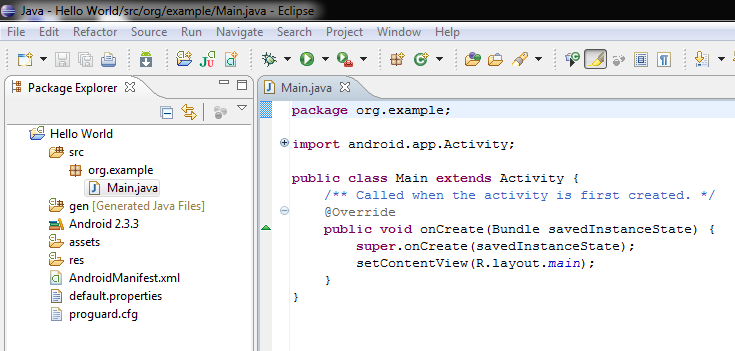
\includegraphics[width=\textwidth]{./images/hello_world_code.png}%
  \caption{Default Hello World code}
  \label{fig:hello_world_code}
\end{figure}

Congratulations, you've now got a working development environment!

\subsection{DDMS}

A key feature is the ability to view what's happening on the device (real or virtual) at any given time. Eclipse has \emph{perspectives} that enable developers to group a series of panes together (by default you're in the `Java' perspective). You can change perspectives by using the menu on the top-right (highlighted in \ref{fig:perspectives}). Select DDMS from the list. 

\begin{figure}[!ht]
  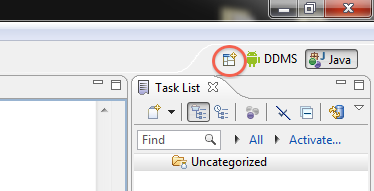
\includegraphics[width=\textwidth]{./images/open_perspective.png}%
  \caption{Opening the DDMS perspective. In this example, it's already been added to the menu bar}
  \label{fig:perspectives}
\end{figure}

You'll see the tools needed to help debug your applications.

\begin{figure*}[!ht]
  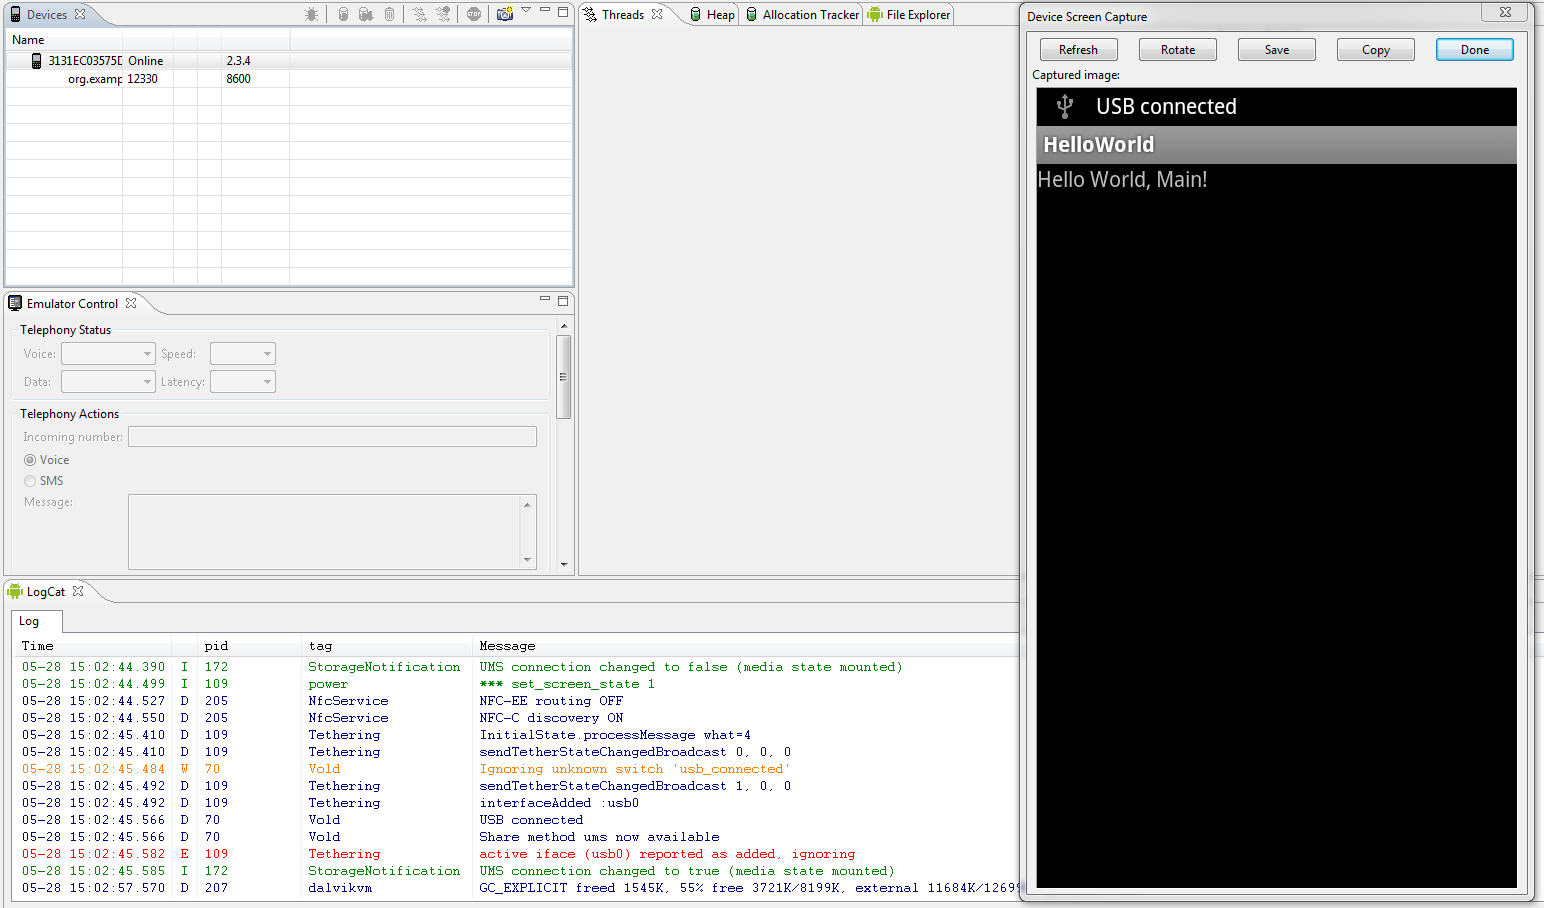
\includegraphics[width=\textwidth]{./images/hello_world_real.png}%
  \caption{Showing DDMS perspective as well as a screen capture from a real device}
  \label{fig:real_hello_world}
\end{figure*}